\documentclass[a4paper,11pt]{article}

% Pacchetti fondamentali
\usepackage[utf8]{inputenc}             % Codifica caratteri
\usepackage{babel}
\babelprovide[import, main]{italian}    % Lingua italiana
\usepackage{amsmath, amssymb}           % Formule matematiche avanzate
\usepackage{graphicx}                   % Inserimento immagini
\usepackage{geometry}                   % Gestione margini
\geometry{margin=2.2cm}
\usepackage{booktabs}                   % Tabelle professionali
\usepackage{physics}
\usepackage{bm}
\usepackage{caption}
\usepackage{textcomp}
\usepackage{parskip}
\usepackage{float}
\usepackage{longtable}
\usepackage{rotating}

% Collegamenti ipertestuali
\usepackage[colorlinks=true, linkcolor=black, urlcolor=blue]{hyperref}

% Dati del documento
\title{\textbf{Misura della curva caratteristica di un diodo semiconduttore in funzione della temperatura}}
\author{\textbf{Studenti:} Bressan Eddi, Feoli Francesco, Rosa Carlotta}
\date{\today}

\begin{document}

\maketitle
\tableofcontents
\newpage

\section{Scopo dell'esperienza}
L'esperienza si prefigge lo studio sperimentale del comportamento elettrico di una giunzione p-n a semiconduttore in differenti condizioni operative e termiche.

\section{Cenni Teorici}
La conduzione in una giunzione $p\text{-}n$ è descritta dall'equazione di Shockley:
\begin{equation*}
    I = I_0 \left( e^{\frac{qV}{\eta k_B T}} - 1 \right)
\end{equation*}
Nei diodi a giunzione in silicio, il fattore di idealità $\eta$ assume tipicamente valori compresi tra 1 e 2.

Per tensioni di polarizzazione diretta ($V \gg \frac{\eta k_B T}{q}$), l'unità nell'esponenziale è trascurabile. Applicando il logaritmo naturale si ottiene la relazione lineare utilizzata per il semilog:
\begin{equation*}
    \ln(I) \simeq \ln(I_0) + \frac{q}{\eta k_B T} V
\end{equation*}
che rappresenta una retta nel piano $\ln(I)$ vs $V$ con intercetta $\ln(I_0)$. Dalla pendenza $m = \frac{q}{\eta k_B T}$ del fit lineare si ricava il coefficiente $\eta = \frac{q}{k_B T \cdot m}$.

Fissando un valore costante di corrente $I = I^*$, la tensione ai capi della giunzione varia in modo lineare e decrescente con la temperatura assoluta:
\begin{equation*}
    V(T) \simeq V_0 - \alpha T
\end{equation*}
dove la pendenza $-\alpha = \left( \frac{dV}{dT} \right)_{I^*}$ esprime la sensibilità termica del dispositivo.

\section{Setup Sperimentale e Strumentazione}

Il circuito di misura è stato realizzato collegando in serie un generatore di tensione continua regolabile, una resistenza di zavorra $R$ (necessaria a limitare la corrente e proteggere la giunzione), un deviatore per invertire la polarità del circuito e un amperometro. Il voltmetro è stato posto direttamente in parallelo ai reofori del diodo semiconduttore per misurare l'effettiva differenza di potenziale ai suoi capi.

Per il controllo termico, il diodo è stato avvolto in strati di mylar a stretto contatto con la giunzione di una termocoppia per garantirne l'impermeabilizzazione senza alterare il contatto termico, e immerso nei diversi bagni di termostatazione (acqua a temperature controllate tra circa $63\,^\circ\text{C}$ e $2\,^\circ\text{C}$, e azoto liquido a $77.36\text{ K}$).

\textbf{Strumentazione utilizzata:}
\begin{itemize}
    \item Diodo semiconduttore al silicio;
    \item Resistenza limitatrice di carico $R$;
    \item Generatore di tensione continua a bassa tensione;
    \item Tre multimetri digitali (impiegati rispettivamente come voltmetro, amperometro e termometro);
    \item Contenitori per liquidi di termostatazione (bagno d'acqua calda, miscela acqua-ghiaccio e criostato ad azoto liquido);
    \item Fogli di mylar per l'isolamento del sensore e del componente;
    \item Cavetti di rame e morsetti di collegamento.
\end{itemize}

\section{Dati Sperimentali}
Le incertezze associate alle misure dirette di tensione, corrente e temperatura sono state assunte pari alla sensibilità (risoluzione dell'ultimo digit) dei rispettivi multimetri digitali impiegati sul fondo-scala attivo, trattandosi di singole letture non ripetute:
\begin{itemize}
    \item Tensione diretta: $\Delta V = 0.001\text{ V}$;
    \item Corrente diretta: $\Delta I = 0.01\text{ mA}$;
    \item Temperatura: $\Delta T = 0.1\text{ K}$;
    \item Polarizzazione inversa: $\Delta V_{\text{rev}} = 0.001\text{ V}$ (per $V < 4\text{ V}$) e $0.01\text{ V}$ (per $V \ge 4\text{ V}$), $\Delta I_{\text{rev}} = 0.1\ \mu\text{A}$.
\end{itemize}

Dato che l'entità di tali incertezze strumentali risulta inferiore all'ingombro visivo dei punti sperimentali nei grafici, si è scelto di omettere le barre d'errore per preservare la chiarezza grafica e la leggibilità degli andamenti. \\
Le serie complete dei dati grezzi acquisiti per le curve caratteristiche in polarizzazione diretta alle 6 temperature operative ($63.1\,^\circ\text{C}$, $52.8\,^\circ\text{C}$, $41.1\,^\circ\text{C}$, $28.6\,^\circ\text{C}$, $2.0\,^\circ\text{C}$ e azoto liquido a $77.36\text{ K}$) sono riportate integralmente in Appendice per non appesantire la lettura del testo.


\section{Analisi Dati e Grafici}

In Figura \ref{fig:iv_diretta} sono riportate le curve caratteristiche $I-V$ in polarizzazione diretta per le sei temperature studiate. Si nota chiaramente il comportamento esponenziale della corrente all'aumentare della tensione e la progressiva traslazione delle curve verso tensioni più elevate al diminuire della temperatura, con la tensione di soglia che sale fino a circa $1\text{ V}$ alle temperature dell'azoto liquido ($77.36\text{ K}$).

\begin{figure}[H]
    \centering
    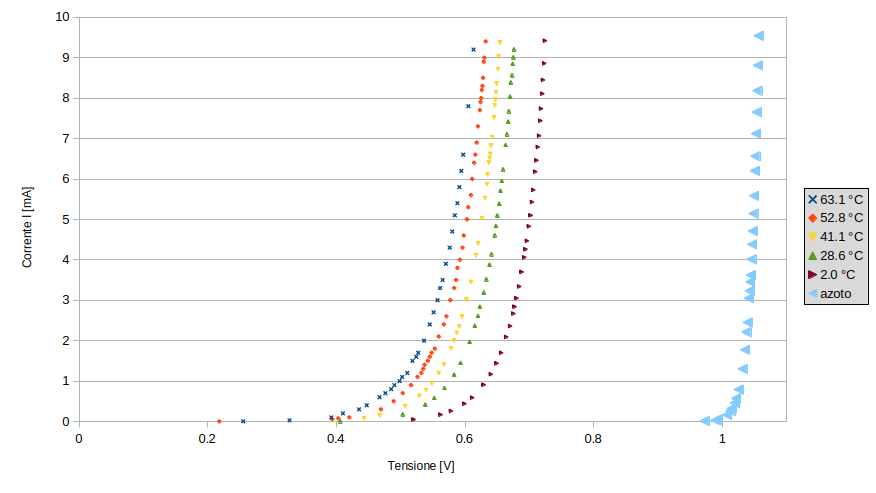
\includegraphics[width=0.85\textwidth]{img/I-V_completo.png}
    \caption{Caratteristiche corrente-tensione $I-V$ del diodo al silicio in polarizzazione diretta per le sei diverse temperature operative.}
    \label{fig:iv_diretta}
\end{figure}

Per linearizzare il comportamento esponenziale e ricavare il parametro di idealità $\eta$, i dati sono stati rappresentati nel piano semilogaritmico $\ln(I)$ vs $V$ (Figura \ref{fig:semilog}), limitando il fit lineare all'intervallo di correnti intermedie in cui la conduzione rispetta l'approssimazione esponenziale pura.

\begin{figure}[H]
    \centering
    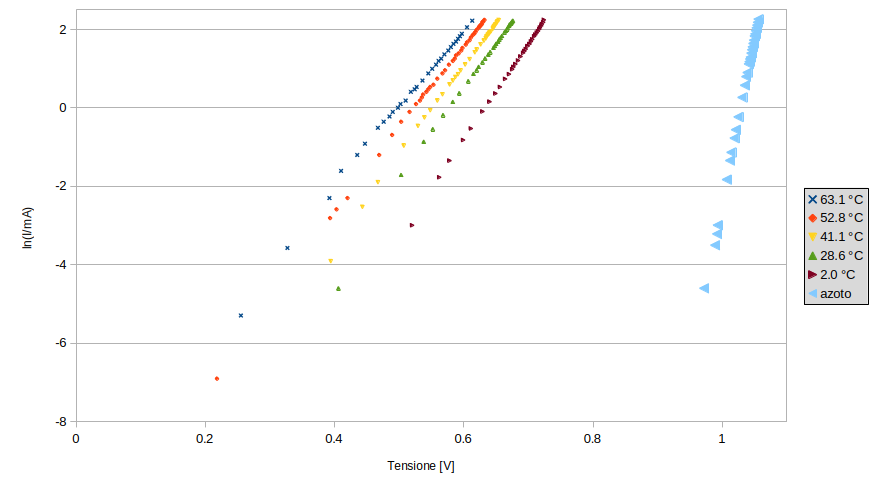
\includegraphics[width=0.85\textwidth]{img/grafico_log.png}
    \caption{Caratteristiche semilogaritmiche $\ln(I)$ in funzione della tensione $V$ con relativi fit lineari per la stima del fattore di idealità $\eta$.}
    \label{fig:semilog}
\end{figure}

Dalla pendenza $m$ di ciascuna retta di fit è stato calcolato il rispettivo fattore $\eta = \frac{q}{k_B T \cdot m}$, riportato in Tabella \ref{tab:eta}.

\begin{table}[H]
\centering
\caption{Valori del coefficiente angolare $m$ del fit semilogaritmico e fattore di idealità $\eta$ calcolato alle diverse temperature operative.}
\label{tab:eta}
\begin{tabular}{|c|c|c|}
\hline
$T\text{ [K]}$ & $m\text{ [V}^{-1}\text{]}$ & $\eta$ \\
\hline
336.25 & 19.16 & 1.80 \\
325.95 & 20.11 & 1.77 \\
314.25 & 21.44 & 1.72 \\
301.75 & 22.13 & 1.74 \\
275.15 & 24.18 & 1.74 \\
77.36  & 81.92 & 1.83 \\
\hline
\end{tabular}
\end{table}

I valori di $\eta$ ottenuti risultano compresi nell'intervallo teorico $1 \le \eta \le 2$ previsto per giunzioni in silicio, indicando la compresenza di correnti di diffusione e ricombinazione nella regione di carica spaziale. Il valore medio campionario risulta pari a $\bar{\eta} = 1.77 \pm 0.04$, confermando l'assunzione di sostanziale costanza del fattore di idealità al variare della temperatura.

In Figura \ref{fig:inversa} è illustrata la caratteristica ottenuta in polarizzazione inversa a temperatura ambiente ($T = 28.4\,^\circ\text{C}$). 

\begin{figure}[H]
    \centering
    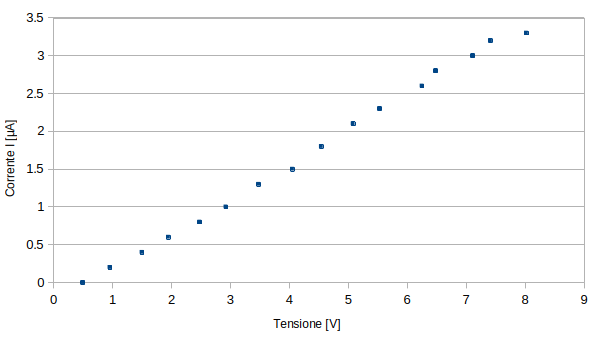
\includegraphics[width=0.85\textwidth]{img/polarita_inversa.png}
    \caption{Caratteristica corrente-tensione in polarizzazione inversa a temperatura ambiente ($T = 28.4\,^\circ\text{C}$).}
    \label{fig:inversa}
\end{figure}

La corrente misurata si attesta nell'ordine dei microampere, sensibilmente superiore al valore teorico ideale di saturazione $I_0$ (tipicamente compreso tra picoampere e nanoampere). Tale discrepanza è legata sia alle correnti di dispersione superficiale lungo il bordo della giunzione, sia all'effetto di carico introdotto dalla resistenza interna finita del voltmetro digitale ($R_V \approx 10\text{ M}\Omega$) posto in parallelo al diodo.

Fissando infine tre valori di corrente ($2\text{ mA}$, $4\text{ mA}$, $6\text{ mA}$), è stata valutata la tensione $V$ in funzione di $T$ (Figura \ref{fig:vt_costante}).

\begin{figure}[H]
    \centering
    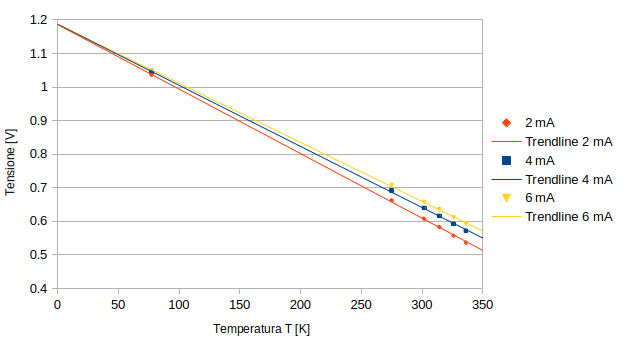
\includegraphics[width=0.85\textwidth]{img/grafico_fit.png}
    \caption{Andamento della tensione $V$ in funzione della temperatura $T$ a correnti fissate ($2\text{ mA}$, $4\text{ mA}$, $6\text{ mA}$) con estrapolazione lineare allo zero assoluto.}
    \label{fig:vt_costante}
\end{figure}

L'estrapolazione lineare delle rette verso lo zero assoluto ($T \to 0\text{ K}$) fornisce intercette comprese tra circa $1.18\text{ V}$ e $1.20\text{ V}$, coerenti con l'ampiezza di banda proibita $E_g(0)/q \approx 1.17 - 1.21\text{ V}$.

\section{Conclusioni}

L'indagine sperimentale condotta sulla giunzione $p\text{-}n$ ha consentito di verificare accuratamente i modelli teorici di conduzione e la dipendenza termica del dispositivo.

\begin{itemize}
    \item \textbf{Caratteristica in polarizzazione diretta e fattore di idealità:} Le curve $I-V$ rilevate confermano il previsto andamento esponenziale della corrente con la tensione. L'analisi semilogaritmica condotta sulle sei temperature ha fornito un fattore di idealità medio pari a:
    \begin{equation*}
        \bar{\eta} = 1.77 \pm 0.04
    \end{equation*}
    Tale risultato si colloca stabilmente nell'intervallo teorico atteso ($1 \le \eta \le 2$), evidenziando come nei processi di conduzione del dispositivo concorrano sia correnti diffusive sia meccanismi di ricombinazione nella zona di svuotamento.

    \item \textbf{Sensibilità termica e determinazione del materiale:} L'analisi della tensione ai capi della giunzione a correnti costanti in funzione della temperatura ($V$ vs $T$) ha confermato la linearità prevista dal modello teorico, attestando la sensibilità termica del componente a coefficienti compresi tra $-1.76\text{ mV/K}$ e $-1.92\text{ mV/K}$. L'estrapolazione lineare delle caratteristiche allo zero assoluto ($T \to 0\text{ K}$) restituisce un potenziale di gap:
    \begin{equation*}
        V_G \approx 1.18 - 1.20\text{ V}
    \end{equation*}
    Il valore ottenuto risulta in ottimo accordo con il potenziale di gap teorico del silicio a $0\text{ K}$ ($V_G \simeq 1.21\text{ V}$), escludendo categoricamente semiconduttori alternativi quali il germanio ($V_G \simeq 0.785\text{ V}$) e identificando senza ambiguità la natura del materiale impiegato.

    \item \textbf{Polarizzazione inversa:} Il comportamento asimmetrico della giunzione è stato verificato in regime di polarizzazione inversa. La discrepanza riscontrata tra la corrente misurata (ordine dei $\mu\text{A}$) e il valore asintotico teorico di saturazione $I_0$ è pienamente imputabile alle correnti di conduzione superficiale e alla resistenza ohmica interna finita dello strumento di misura posto in parallelo ($R_V \approx 10\text{ M}\Omega$).
\end{itemize}

\newpage
\appendix
\section{Dati Sperimentali Completi}
\label{sec:appendice_dati}

In questa sezione sono raccolte le serie complete delle misurazioni di tensione diretta $V$ e corrente $I$ acquisite per le sei temperature di termostatazione analizzate, oltre ai dati rilevati in regime di polarizzazione inversa.
\begin{table}[H]
\centering
\caption{Dati sperimentali completi di tensione diretta $V$ e corrente $I$ rilevati alle sei temperature analizzate.}
\label{tab:dati_completi_tutte}
\resizebox{\textwidth}{!}{%
\begin{tabular}{|cc|cc|cc|cc|cc|cc|}
\hline
\multicolumn{2}{|c|}{\textbf{63.1 $^\circ$C (336.25 K)}} & 
\multicolumn{2}{c|}{\textbf{52.8 $^\circ$C (325.95 K)}} & 
\multicolumn{2}{c|}{\textbf{41.1 $^\circ$C (314.25 K)}} & 
\multicolumn{2}{c|}{\textbf{28.6 $^\circ$C (301.75 K)}} & 
\multicolumn{2}{c|}{\textbf{2.0 $^\circ$C (275.15 K)}} & 
\multicolumn{2}{c|}{\textbf{Azoto (77.36 K)}} \\
$V\text{ [V]}$ & $I\text{ [mA]}$ & 
$V\text{ [V]}$ & $I\text{ [mA]}$ & 
$V\text{ [V]}$ & $I\text{ [mA]}$ & 
$V\text{ [V]}$ & $I\text{ [mA]}$ & 
$V\text{ [V]}$ & $I\text{ [mA]}$ & 
$V\text{ [V]}$ & $I\text{ [mA]}$ \\
\hline
0.613 & 9.2 & 0.632 & 9.4 & 0.654 & 9.37 & 0.676 & 9.21 & 0.724 & 9.42 & 1.056 & 9.54 \\
0.605 & 7.8 & 0.630 & 9.0 & 0.652 & 9.03 & 0.675 & 9.01 & 0.723 & 8.86 & 1.055 & 8.81 \\
0.597 & 6.6 & 0.629 & 8.9 & 0.651 & 8.72 & 0.674 & 8.85 & 0.721 & 8.45 & 1.054 & 8.18 \\
0.594 & 6.2 & 0.628 & 8.5 & 0.649 & 8.36 & 0.673 & 8.57 & 0.720 & 8.11 & 1.053 & 7.65 \\
0.591 & 5.8 & 0.627 & 8.3 & 0.648 & 8.14 & 0.671 & 8.39 & 0.718 & 7.74 & 1.052 & 7.12 \\
0.588 & 5.4 & 0.626 & 8.2 & 0.647 & 7.96 & 0.670 & 8.04 & 0.717 & 7.44 & 1.051 & 6.56 \\
0.584 & 5.1 & 0.625 & 8.0 & 0.646 & 7.82 & 0.668 & 7.68 & 0.715 & 7.07 & 1.050 & 6.20 \\
0.580 & 4.7 & 0.624 & 7.9 & 0.645 & 7.52 & 0.667 & 7.42 & 0.713 & 6.79 & 1.049 & 5.58 \\
0.576 & 4.3 & 0.623 & 7.7 & 0.642 & 7.03 & 0.665 & 7.11 & 0.711 & 6.46 & 1.048 & 5.14 \\
0.570 & 3.9 & 0.620 & 7.3 & 0.640 & 6.82 & 0.663 & 6.84 & 0.709 & 6.18 & 1.047 & 4.71 \\
0.565 & 3.5 & 0.618 & 6.9 & 0.639 & 6.62 & 0.659 & 6.24 & 0.706 & 5.73 & 1.046 & 4.38 \\
0.561 & 3.3 & 0.616 & 6.6 & 0.638 & 6.52 & 0.657 & 5.95 & 0.704 & 5.43 & 1.045 & 4.01 \\
0.557 & 3.0 & 0.614 & 6.4 & 0.637 & 6.40 & 0.655 & 5.71 & 0.702 & 5.10 & 1.044 & 3.62 \\
0.551 & 2.7 & 0.611 & 6.0 & 0.635 & 6.11 & 0.653 & 5.39 & 0.699 & 4.83 & 1.043 & 3.45 \\
0.545 & 2.4 & 0.609 & 5.6 & 0.634 & 5.87 & 0.650 & 5.10 & 0.696 & 4.47 & 1.042 & 3.23 \\
0.536 & 2.0 & 0.605 & 5.3 & 0.631 & 5.53 & 0.648 & 4.84 & 0.694 & 4.26 & 1.041 & 3.05 \\
0.527 & 1.7 & 0.603 & 5.0 & 0.626 & 5.03 & 0.646 & 4.61 & 0.692 & 4.06 & 1.039 & 2.45 \\
0.524 & 1.6 & 0.598 & 4.6 & 0.620 & 4.40 & 0.641 & 4.14 & 0.688 & 3.70 & 1.037 & 2.21 \\
0.518 & 1.5 & 0.596 & 4.3 & 0.617 & 4.11 & 0.638 & 3.88 & 0.684 & 3.34 & 1.035 & 1.77 \\
0.510 & 1.2 & 0.592 & 4.0 & 0.609 & 3.45 & 0.633 & 3.52 & 0.680 & 3.05 & 1.031 & 1.30 \\
0.502 & 1.1 & 0.588 & 3.8 & 0.602 & 3.01 & 0.629 & 3.19 & 0.677 & 2.84 & 1.025 & 0.79 \\
0.498 & 1.0 & 0.586 & 3.5 & 0.595 & 2.59 & 0.623 & 2.84 & 0.675 & 2.67 & 1.021 & 0.57 \\
0.490 & 0.9 & 0.583 & 3.3 & 0.591 & 2.35 & 0.620 & 2.61 & 0.670 & 2.36 & 1.019 & 0.46 \\
0.485 & 0.8 & 0.577 & 3.0 & 0.587 & 2.19 & 0.615 & 2.37 & 0.664 & 2.09 & 1.014 & 0.32 \\
0.476 & 0.7 & 0.571 & 2.6 & 0.583 & 2.00 & 0.607 & 1.97 & 0.656 & 1.70 & 1.012 & 0.26 \\
0.467 & 0.6 & 0.567 & 2.4 & 0.578 & 1.81 & 0.593 & 1.45 & 0.649 & 1.44 & 1.007 & 0.16 \\
0.447 & 0.4 & 0.559 & 2.1 & 0.567 & 1.41 & 0.583 & 1.16 & 0.640 & 1.17 & 0.993 & 0.05 \\
0.435 & 0.3 & 0.553 & 1.8 & 0.559 & 1.20 & 0.568 & 0.83 & 0.629 & 0.91 & 0.992 & 0.04 \\
0.410 & 0.2 & 0.548 & 1.7 & 0.548 & 0.94 & 0.552 & 0.58 & 0.611 & 0.59 & 0.989 & 0.03 \\
0.392 & 0.1 & 0.545 & 1.6 & 0.539 & 0.78 & 0.538 & 0.42 & 0.599 & 0.44 & 0.972 & 0.01 \\
0.327 & 0.0280 & 0.542 & 1.5 & 0.529 & 0.63 & 0.503 & 0.18 & 0.578 & 0.26 & -- & -- \\
0.255 & 0.0050 & 0.537 & 1.4 & 0.507 & 0.38 & 0.406 & 0.01 & 0.562 & 0.17 & -- & -- \\
-- & -- & 0.535 & 1.3 & 0.467 & 0.15 & -- & -- & 0.520 & 0.05 & -- & -- \\
-- & -- & 0.532 & 1.2 & 0.443 & 0.08 & -- & -- & -- & -- & -- & -- \\
-- & -- & 0.526 & 1.1 & 0.394 & 0.02 & -- & -- & -- & -- & -- & -- \\
-- & -- & 0.516 & 0.9 & -- & -- & -- & -- & -- & -- & -- & -- \\
-- & -- & 0.503 & 0.7 & -- & -- & -- & -- & -- & -- & -- & -- \\
-- & -- & 0.489 & 0.5 & -- & -- & -- & -- & -- & -- & -- & -- \\
-- & -- & 0.469 & 0.3 & -- & -- & -- & -- & -- & -- & -- & -- \\
-- & -- & 0.420 & 0.1 & -- & -- & -- & -- & -- & -- & -- & -- \\
-- & -- & 0.403 & 0.075 & -- & -- & -- & -- & -- & -- & -- & -- \\
-- & -- & 0.393 & 0.060 & -- & -- & -- & -- & -- & -- & -- & -- \\
-- & -- & 0.218 & 0.001 & -- & -- & -- & -- & -- & -- & -- & -- \\
\hline
\end{tabular}%
}
\end{table}


\begin{table}[H]
\centering
\caption{Dati sperimentali in polarizzazione inversa a temperatura ambiente ($T = 28.4\,^\circ\text{C}$).}
\label{tab:dati_inversa}
\begin{tabular}{|c|c|c|c|}
\hline
$V_{\text{rev}}\text{ [V]}$ & $\Delta V\text{ [V]}$ & $I_{\text{rev}}\text{ [}\mu\text{A]}$ & $\Delta I\text{ [}\mu\text{A]}$ \\
\hline
0.492 & 0.001 & 0.0 & 0.1 \\
0.953 & 0.001 & 0.2 & 0.1 \\
1.497 & 0.001 & 0.4 & 0.1 \\
1.945 & 0.001 & 0.6 & 0.1 \\
2.477 & 0.001 & 0.8 & 0.1 \\
2.921 & 0.001 & 1.0 & 0.1 \\
3.476 & 0.001 & 1.3 & 0.1 \\
4.05  & 0.01  & 1.5 & 0.1 \\
4.54  & 0.01  & 1.8 & 0.1 \\
5.08  & 0.01  & 2.1 & 0.1 \\
5.53  & 0.01  & 2.3 & 0.1 \\
6.25  & 0.01  & 2.6 & 0.1 \\
6.48  & 0.01  & 2.8 & 0.1 \\
7.11  & 0.01  & 3.0 & 0.1 \\
7.41  & 0.01  & 3.2 & 0.1 \\
8.02  & 0.01  & 3.3 & 0.1 \\
\hline
\end{tabular}
\end{table}
\end{document}